%!TEX root = ../doc.tex
\chapter{Konzept}
\label{sec:konzept}

Aus den Anforderungen ist klar ersichtlich dass eine eigene Benutzeroberfläche entwickelt werden soll, welche über die Programmierschnittstelle von LoBo kommunizieren soll. Die nicht funktionelle Anforderung NFREQ-001 verlangt eine Web Browser kompatible Benutzeroberfläche und disqualifiziert eine zu installierende Desktop Client Anwendung. Trotz der Limitierung der Lösungsmöglichkeiten, bleiben bei der Entwicklung einer Benutzeroberfläche im Web viele Fragen offen. Im folgenden werden die Technologie- sowie Architekturentscheidungen vorgestellt und begründet.

\section{Web Modell}
Traditionelle Websites bestehen aus mehreren \textit{Hyper Text Markup Language} (HTML) Seiten und liefern diese, wenn der Client sie anfordert aus. Es gibt verschiedene Programmiersprachen welche es erlauben zum Zeitpunkt des Aufrufs, Code welcher in diesen HTML Seiten vorhanden ist zu interpretieren und des entsprechende Resultat auszuliefern. \textit{PHP Hypertext Preprocessor}\footnote{Offizielle Website von PHP: \url{http://php.net/}} (PHP) ist eine der bekanntesten Programmiersprachen. Aber auch Python bietet mit dem Framework \textit{Django}\footnote{Offizielle Website von Django: \url{https://www.djangoproject.com}} eine ähnliche Funktionalität an. Mit der zunehmende Möglichkeiten im Web sowie der immer grösseren Komplexität wurden andere Modelle für das Web entwickelt. Mit der offiziellen Spezifikation des \textit{XMLHttpRequest Object} am 5. April 2006\citep[]{w3cXMLHttpRequest} und dessen Einsatz von Google in Webapplikationen wie Gmail und Google Maps, wurde die Entwicklung von \textit{Single-page application} (SPA) ermöglicht. Mit \textit{XMLHttpRequest} ist es möglich nach dem Laden der Website eine Anfrage an den Server zu schicken ohne dabei die Gesamte HTML Seite neu zu laden. Für die Ausführung dieser \textit{XMLHttpRequest} Anfragen wird eine clientseitige Skriptsprache benötigt. Trotz vereinzelten Alternativen ist JavaScript der Standard bei den browserfähigen clientseitigen Skriptsprachen. Dies ist mitunter auch ein Grund warum SPA Webseiten mit JavaScript erstellt werden. In der Abbildung \ref{fig:ajax}\footnote{Author: DanielSHaischt, Lizenz: CC BY-SA 3.0, Link: \url{https://en.wikipedia.org/wiki/Ajax_(programming)#/media/File:Ajax-vergleich-en.svg}} ist der Unterschied zwischen einer traditionellen und einer \textit{XMLHttpRequest} Anfrage veranschaulicht.

\subsection{Single-page application}
\textit{Single-page application} (SPA) haben viele Vorteile gegenüber traditionellen Webseiten. Die Gesamte Webseite kann mit nur drei Anfragen (1. HTML Seite, 2. Cascading Style Sheets (CSS), 3. JavaScript) an den Server geladen werden. Alle weiteren DAten wie z.B. Benutzerdaten aus der Datenbank werden asynchron mit einer \textit{XMLHttpRequest} Anfrage, während die Webseite im Browser aufgebaut wird geladen. Dies hat den Vorteil dass die Webseite bedeutend schneller geladen wird und der trägt zur Benutzerfreundlichkeit bei. Im folgende ist eine nicht abgeschlossene Liste mit den Vorteilen von SPA.
\begin{description}
	\item[Entkopplung Daten / Business Logic / UI]
	\item[Entlastung des Server]
	\item[Performant (weniger traffic)]
\end{description}

\begin{figure}[ht]
	\centering
  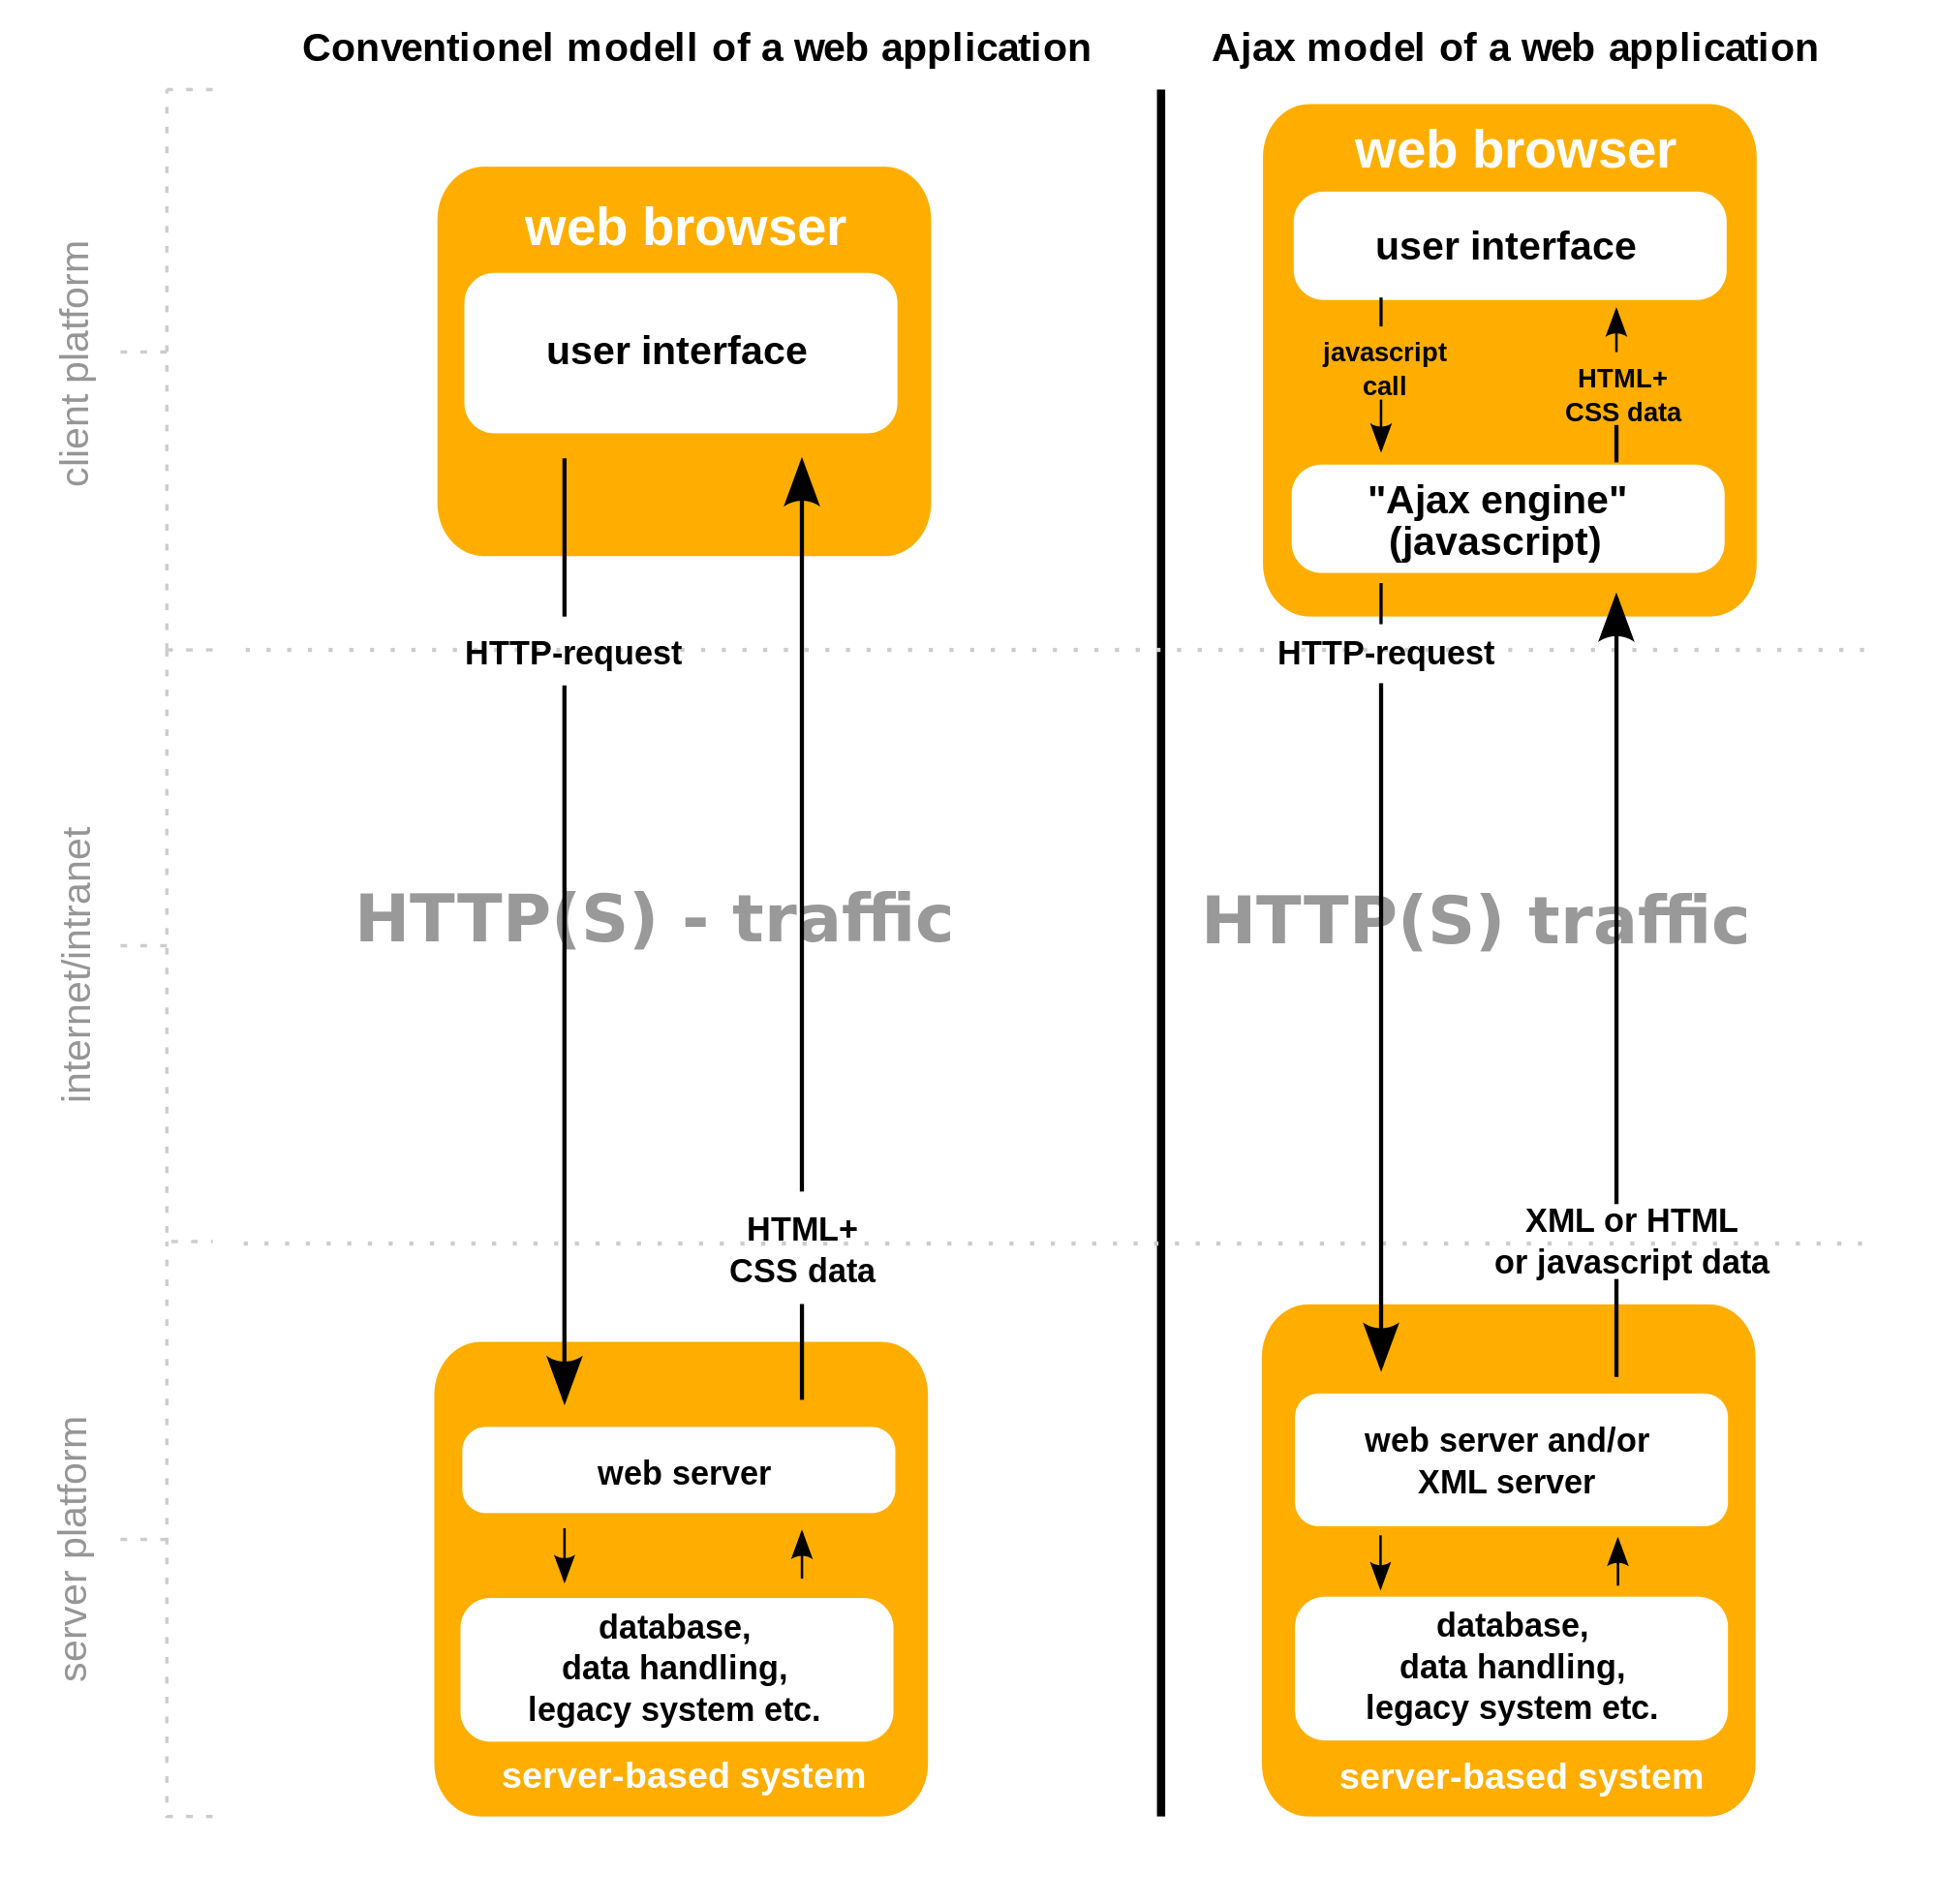
\includegraphics[width=0.88\textwidth]{images/ajax.png}
	\caption{Visualisierung einer XMLHttpRequest und einer traditionellen Anfrage}
	\label{fig:ajax}
\end{figure}



\section{Planung}
Möglichkeit 1: JS client direkt auf LOBO und (andere services) -> security / performance bottelneck weil immer gleiche Lobo Instanz

Möglichkeit 2: JS client mit mini Backend (zurzeit notwendige Business logik weg von frontend, Secure (API Keys), mini backend instanzen sind einfach hoch zu skalieren (weil keine DB.)

Progressive Web App -> JavaScript (sehr populäre sprache und bietet am meisten möglichkeiten)
Single Page App -> momentaner Standard, grosser erfolgfaktor bei Benutzererfahrung.  Lässt abtrennung zwischen Business Logik und UI/UX Logik zu. Aufgaben aufteilung

Nodejs -> weil gleiche Programmiersprache für Front und Back. JSON!!! einfach und adaptiv für features welche schlussendlich in Lobo implementiert werden sollen.

ES2015 -> weil besser performance mit weniger libs. Neuer standard. besser maintainbarer code

FLux -> weil Prozess weniger störungs anfällig, immer klarer State,
https://scotch.io/tutorials/getting-to-know-flux-the-react-js-architecture

React -> weil Flux, weil slim, weil Komponenten (wiederverwendbarkeit), weil brand neu

Addresse Auto Complete -> Google Maps and Open street maps
Sbb times -> opendata.ch



%http://iso4app.net/ für die polygone
%https://github.com/tmpvar/polygon.js
%https://www.npmjs.com/package/vec2


%https://www.smashingmagazine.com/2016/06/an-introduction-to-redux/?utm_source=javascriptweekly&utm_medium=email

\section{Schnittstellen}
\section{Technologie}
\section{Architektur}

\subsection{Frontend}
Alle actions wie adresse auto complete, update stop info, update task info in komponenten. können in Steps und Advanced tour wiederverwendet werden. Steps sind auch wieder komponenten welche die anderen komponenten weiderverwenden.

\subsection{Backend}
Frontend ausliefern und API

Api notwendigen aufrufe. Nur notwendigstes zurück liefern. Error handling wenn möglich nur im Backend.
